\documentclass[conference]{IEEEtran}
\IEEEoverridecommandlockouts
% The preceding line is only needed to identify funding in the first footnote. If that is unneeded, please comment it out.
\usepackage{cite}
\usepackage{url}
\usepackage{amsmath,amssymb,amsfonts}

\usepackage{graphicx}
\usepackage{textcomp}
\usepackage{xcolor}
\usepackage{algorithm}
\usepackage{algpseudocode}
\usepackage{float}
\usepackage{booktabs}
\def\BibTeX{{\rm B\kern-.05em{\sc i\kern-.025em b}\kern-.08em
    T\kern-.1667em\lower.7ex\hbox{E}\kern-.125emX}}
\begin{document}

\title{Operation Theater Planning Using Stochastic Programming and SAA\\
}

\author{\IEEEauthorblockN{1\textsuperscript{st} Jurgen van der Blom}
\IEEEauthorblockA{
j.j.vanderblom@student.utwente.nl}
\and
\IEEEauthorblockN{2\textsuperscript{nd} Eric (H.Q.) van Ree}
\IEEEauthorblockA{
h.q.vanree@student.utwente.nl}
}

\maketitle

\section{Introduction}
Operating room (OR) and Operating theater (OT) planning and scheduling are central topics in healthcare operations research because the operating theater is often considered as one of the hospital's most resource-intensive and operationally critical environments. Efficient scheduling has direct implications for patient access, service quality, staff utilization, and hospital cost control. In literature, these planning problems are categorized in multiple decision levels, such as strategical, tactical and operational \cite{guerriero-2010}. \cite{CARDOEN2010921} reviews the literature based on problem characteristics. 

A key difficulty in OT scheduling is that surgery durations are inherently uncertain. Deterministic schedules based only on expected durations often perform poorly in practice, since deviations in realized procedure times propagate throughout the day and lead to patient waiting, downstream idle time, and overtime. Recent literature therefore increasingly models OR scheduling as an optimization problem under uncertainty.

In this research, an operational OT planning is made using mixed integer programming and sample average approximation. We study a weekly surgery scheduling problem for a set of inpatients that must be assigned to OT sessions, sequenced within each session, and given planned start times that are communicated in advance to the wards. The scheduling objective is to minimize a weighted sum of patient waiting time, OT idle time, and OT overtime, while respecting practical constraints such as fixed OT opening times, deterministic changeover times, and the operational requirement that patients cannot be brought to the OT before their announced start times. From a modeling perspective, this problem integrates assignment, sequencing, and timing decisions in a stochastic environment.

\section{Literature review}
The contribution of this report is to formulate the problem as a stochastic programming model and to evaluate its performance using a finite scenario set generated through sample average approximation (SAA). In this chapter, we will identify an appropriate solution approach and introduce the sample average approximation approach. 

\subsection{Solution approaches}
\subsubsection{Advance and allocation steps}
In literature, the advance and allocation steps can be solved using either sequential (SEQ) or integrated (INT) approaches \cite{Molina-Pariente2026}. Typically, the SEQ approach addresses the advance scheduling and allocation scheduling steps sequentially, whereas with the integrated approach, both advance and allocation steps are jointly addressed.

\textbf{Sequential Approach:}
Dai et al. propose a mathematical formulation to model surgery schedules under uncertainty of surgery duration in which patients are assigned to an operating room and place in the sequence of patients within the operation room \cite{DAI2025107098}.
In \cite{Denton2006} the one operation room problem is formulated as a two-stage stochastic mixed-integer-program, where the first state decision variables include the sequence of operations and planned starting time and the second stage decision variables include the idletime, overtime and waitingtime.

\textbf{Integrated Approach:}
\cite{Moosavi2018216} propose an integrated approach in which another index for the pre-defined number of slots available within a block is included in the decision variable such that a patient is assigned a day, session, and timeslot within the session. \cite{Vali-Siar2018549} uses a binary variable for whether a patient (p) is scheduled in OR (o) with surgeon (s) at time (t) on day (d). 

\subsubsection{Open (OS) and Block (BS) Scheduling}
Traditionally, open (OS) and block (BS) scheduling policies are considered in the literature. Under the OS policy, any surgeon can perform surgeries in any OR-day available within the planning horizon, which complicates the problem. A variant of the OS policy, the BS policy, is therefore frequently used in reality. With the BS policy, a surgeon only performs surgeries in one OR block time. In this case, the determination of the start times is simplified compared with the OS policy as it allows OR-sessions to be scheduled separately. 

To regard the advance and allocation steps, the sequential approach allows modelling the problem in a way that does not require pre-defining a total number of slots per session whhich is preferred given the problem at hand in which patient treatments durations differ significantly, such that it might require introducing dummy patients to fill all patient slots, depending on the model. In addition, the problem is dealt with as a block scheduling problem, in which blocks are separately sequenced to simplify the problem at hand. 

\subsection{Sample average approximation}
In the paper of Molina-Pariente et al. \cite{Molina-Pariente2026} an integrated operating room planning and scheduling problem under uncertainty is discussed. The model is formulated by denoting a set of days H (planning horizon) and a set J of ORs ($j=1,...,|J|)$ available on each day h in the planning horizon, denoting (j,h) as OR-day. To solve the problem, the sample average approximation (SAA) procedure, in which the problem is approximated as a discrete deterministic problem that integrates N samples, is proposed. \cite{Denton2006} also proposes SAA to solve the problem at hand. The SAA approach \cite{Kleywegt} follows the logic described in algorithm \ref{alg:saa} and is a good solution methodology for problems in which numerous different outcomes may occur, such that an exact solution becomes computationally intractable. \textbf{For such problems, stochastic programming using SAA is a good way to balance computational complexity and the solution quality by considering various scenarios all at once, as if it were deterministic. The disadvantage is that the solution quality solely depends on how well the used scenarios represenet the potential outcomes. In the SAA design, a proper sampling method as well as an appropiate sample size (which balances computational requirements and outcome coverage) should be determined for the matematical model. In addition, an appropiate evaluation sample should be determined to evaluate the solution quality upon. ~"show why SP with SAA is a good solution methodology for this problem" "From this review it should be clear why SAA is suitable for the problems at hand, what the disadvantages are, which design choices should be made, and a step-by-step approach on how you will implement SAA in your assignment."}

\begin{algorithm}[H]
\caption{Sample Average Approximation (SAA) Algorithm for Stochastic Discrete Optimization}
\label{alg:saa}
\begin{algorithmic}[1:]
\Statex \textbf{Step 1:}
\State Choose initial sample sizes $N$ (nr. of scenarios) and $N'$ (size of the evaluation sample), a decision rule for determining the number $M$ of SAA replications, a decision rule for increasing the sample sizes $N$ and $N'$ if needed, and tolerance $\varepsilon$.
\Statex \textbf{Step 2:}
\For{$m = 1, \dots, M$}
    \State Generate a sample of size $N$ and solve the SAA problem with objective value $\hat{v}_N^m$ and $\varepsilon$-optimal solution $\hat{x}_N^m$.
    \State Estimate the optimality gap $g(\hat{x}_N^m) - v^*$ and the variance of the gap estimator.
    \If{the optimality gap and the variance of the gap estimator are sufficiently small}
        \State \textbf{go to Step 4}
    \EndIf
\EndFor
\Statex \textbf{Step 3:}
\If{the optimality gap or the variance of the gap estimator is too large}
    \State Increase the sample sizes $N$ and/or $N'$.
    \State Return to Step 2.
\EndIf
\Statex \textbf{Step 4:}
\State Choose the best solution $\hat{x}$ among all candidate solutions $\hat{x}_N^m$ produced, using a screening and selection procedure.
\State \textbf{Stop.}
\end{algorithmic}
\end{algorithm}

\section{Problem description}

\section{Mathematical Model}

\section{SAA procedure}

\section{Results and Evaluation}

\section{Problem Description}

We consider a weekly surgery scheduling problem in a hospital operating theatre 
consisting of multiple ORs. At the start of each week, all 
inpatients $p \in P$ on the waiting list must be scheduled for surgery. The 
scheduling process involves three interrelated decisions: (i)~\textit{assignment} 
of patients to OR sessions, (ii)~\textit{sequencing} of patients within each OR, 
and (iii)~\textit{timing}, i.e., determining the planned start time $S_p$ 
communicated to the wards before the shift begins.

Each OR opens at $t_{\text{open}} = 8{:}00$ h and closes at $t_{\text{close}}$. 
The first patient in every OR begins surgery at opening time. Subsequent patients 
may not start before their communicated planned start time, as ward nurses are 
assumed to be perfectly punctual. A deterministic changeover time of 10 minutes 
is required between any two consecutive surgeries.

The key source of uncertainty is the surgery duration $d_p$, which is unknown at 
the time of scheduling. Because surgeries cannot start 
before their planned start time but may finish later than expected, delays 
propagate through the sequence within an OR session.

The objective is to minimise the weighted sum of three cost components: the total patient waiting time, the total OR idle time , and the 
total overtime. 

Because $d_p$ is continuous and its realisation is only observed after scheduling, 
an exact deterministic formulation is insufficient. We therefore adopt a 
two-stage stochastic programming framework with SAA~\cite{Kleywegt}: First-stage decisions (assignment, 
sequencing, timing) are made before uncertainty is revealed, while second-stage 
costs (start time, waiting, idle, overtime) are evaluated over a finite scenario set. The goal is to find a schedule that minimises 
expected costs across all scenarios. 

\section{Literature review}
The contribution of this report is to formulate the problem as a stochastic programming model and to evaluate its performance using a finite scenario set generated through sample average approximation (SAA). In this chapter, we will identify an appropriate solution approach and introduce the sample average approximation approach. 

\subsection{Solution approaches}
\subsubsection{Advance and allocation steps}
In literature, the advance and allocation steps can be solved using either sequential (SEQ) or integrated (INT) approaches \cite{Molina-Pariente2026}. Typically, the SEQ approach addresses the advance scheduling and allocation scheduling steps sequentially, whereas with the integrated approach, both advance and allocation steps are jointly addressed.

\textbf{Sequential Approach:}
Dai et al. propose a mathematical formulation to model surgery schedules under uncertainty of surgery duration in which patients are assigned to an operating room and place in the sequence of patients within the operation room \cite{DAI2025107098}.
In \cite{Denton2006} the one operation room problem is formulated as a two-stage stochastic mixed-integer-program, where the first state decision variables include the sequence of operations and planned starting time and the second stage decision variables include the idletime, overtime and waitingtime.

\textbf{Integrated Approach:}
\cite{Moosavi2018216} propose an integrated approach in which another index for the pre-defined number of slots available within a block is included in the decision variable such that a patient is assigned a day, session, and timeslot within the session. \cite{Vali-Siar2018549} uses a binary variable for whether a patient (p) is scheduled in OR (o) with surgeon (s) at time (t) on day (d). 

\subsubsection{Open (OS) and Block (BS) Scheduling}
Traditionally, open (OS) and block (BS) scheduling policies are considered in the literature. Under the OS policy, any surgeon can perform surgeries in any OR-day available within the planning horizon, which complicates the problem. A variant of the OS policy, the BS policy, is therefore frequently used in reality. With the BS policy, a surgeon only performs surgeries in one OR block time. In this case, the determination of the start times is simplified compared with the OS policy as it allows OR-sessions to be scheduled separately. 

To regard the advance and allocation steps, the sequential approach allows modelling the problem in a way that does not require pre-defining a total number of slots per session whhich is preferred given the problem at hand in which patient treatments durations differ significantly, such that it might require introducing dummy patients to fill all patient slots, depending on the model. In addition, the problem is dealt with as a block scheduling problem, in which blocks are separately sequenced to simplify the problem at hand. 

\subsection{Sample average approximation}
In the paper of Molina-Pariente et al. \cite{Molina-Pariente2026} an integrated operating room planning and scheduling problem under uncertainty is discussed. The model is formulated by denoting a set of days H (planning horizon) and a set J of ORs ($j=1,...,|J|)$ available on each day h in the planning horizon, denoting (j,h) as OR-day. To solve the problem, the sample average approximation (SAA) procedure, in which the problem is approximated as a discrete deterministic problem that integrates N samples, is proposed. \cite{Denton2006} also proposes SAA to solve the problem at hand. The SAA approach \cite{Kleywegt} follows the logic described in algorithm \ref{alg:saa} and is a good solution methodology for problems in which numerous different outcomes may occur, such that an exact solution becomes computationally intractable. 

Stochastic programming is a good way to balance computational complexity and the solution quality by considering various scenarios all at once, as if it were deterministic. The disadvantage is that the solution quality solely depends on how well the used scenarios represent the potential outcomes. The SAA approach helps determine which minimum number of scenarios, and how to derive these scenarios, is then suitable to cover the outcome space appropriately whilst minimizing computational cost.  The SAA procedure provides a stepwise approach to determine an appropriate number of scenarios ($N$) that balance computational requirements and outcome quality. In the SAA design, a sampling method should be used for generating samples. Generally, random sampling is applied in SAA, but other examples are Latin hypercube, orthogonal, or importance sampling. In addition, an appropiate evaluation sample should be determined to evaluate the solution quality upon. The downside of the SAA approach is that it requires solving the model with $N$ scenarios $M$ times until a suitable $N$ is found. Selection of a proper $N$, $M$ and $N'$ to start with therefore also heavily affects how long the SAA approach takes to perform.



For the surgery scheduling problem at hand, SAA is particularly appropriate
for three reasons.
First, surgery durations follow a continuous lognormal distribution, making the
full stochastic program with its infinite scenario space computationally
intractable; SAA converts it to a tractable finite MILP.
Second, the scenario subproblems are independent — no second-stage constraints
link scenarios to each other — so the deterministic equivalent scales linearly
in the number of scenarios~$N$.
Third, the block scheduling structure means OR sessions can be evaluated
separately, keeping individual subproblem sizes manageable.
The main disadvantage of SAA is that solution quality depends on how well the
$N$ scenarios represent the true distribution: if tail events (long surgeries
causing cascade overtime) are under-sampled, the policy may underestimate
expected cost. This motivates evaluating multiple sampling strategies alongside
random sampling and using a large out-of-sample evaluation set to validate
quality independently of the training sample.

\begin{algorithm}[H]
\caption{Sample Average Approximation (SAA) Algorithm for Stochastic Discrete Optimization}
\label{alg:saa}
\begin{algorithmic}[1:]
\Statex \textbf{Step 1:}
\State Choose initial sample sizes $N$ (nr. of scenarios) and $N'$ (size of the evaluation sample), a decision rule for determining the number $M$ of SAA replications, a decision rule for increasing the sample sizes $N$ and $N'$ if needed, and tolerance $\varepsilon$.
\Statex \textbf{Step 2:}
\For{$m = 1, \dots, M$}
    \State Generate a sample of size $N$ and solve the SAA problem with objective value $\hat{v}_N^m$ and $\varepsilon$-optimal solution $\hat{x}_N^m$.
\State Estimate the optimality gap $g(\hat{x}_N^m) - v^*$ and the variance of the gap estimator.
    \If{the optimality gap and the variance of the gap estimator are sufficiently small}
        \State \textbf{go to Step 4}
    \EndIf
\EndFor
\Statex \textbf{Step 3:}
\If{the optimality gap or the variance of the gap estimator is too large}
    \State Increase the sample sizes $N$ and/or $N'$.
    \State Return to Step 2.
\EndIf
\Statex \textbf{Step 4:}
\State Choose the best solution $\hat{x}$ among all candidate solutions $\hat{x}_N^m$ produced, using a screening and selection procedure.
\State \textbf{Stop.}
\end{algorithmic}
\end{algorithm}
%mathematical model
\section{Mathematical model}
\label{sec:mathematical_model}
In this chapter we introduce the integer linear program used to solve the instances. 
The model is formulated as a two-stage stochastic mixed-integer linear program and
is solved through its deterministic equivalent formulation.

\subsection{Sets and Indices}

\begin{itemize}
  \item $p \in P$ -- set of patients (surgeries)
  \item $P_0 = P \cup \{0\}$ -- patients plus dummy depot node (session start)
  \item $h \in H$ -- set of available OR sessions
  \item $s \in S$ -- set of scenarios
  \item $q \in Q = \{\text{CHI},\text{ORT},\text{KNO}\}$ -- set of surgical
        specialties
\end{itemize}

\subsection{Parameters}

\begin{itemize}
  \item $d_{ps}$ -- surgery duration of patient $p$ in scenario $s$
  \item $\pi_s$ -- probability of scenario $s$,
        where $\sum_{s \in S} \pi_s = 1$
  \item $c$ -- changeover time
  \item $t^{\text{start}}$ -- common session start time (identical for all ORs)
  \item $t^{\text{close}}$ -- common session closing time (identical for all
        ORs)
  \item $q_{pq} \in \{0,1\}$ -- 1 if patient $p$ belongs to specialty $q$
  \item $M$ -- sufficiently large constant (big-$M$)
  \item $\beta_1=0.6, \beta_2=0.2, \beta_3=0.2, \beta_4=100$ -- weights for waiting time, idle
        time, overtime, and specialty mismatch, respectively
\end{itemize}

\subsection{First-Stage Decision Variables}

The following decisions are made before scenario realisation:

\begin{itemize}
  \item $A_p$ -- appointment time assigned to patient $p$
  \item $X_{ijh}$ -- 1 if patient $j$ is scheduled directly after
        patient $i$ in session $h$
  \item $Y_{ph}$ -- 1 if patient $p$ is assigned to session $h$
  \item $Z_h$ -- 1 if OR session $h$ is opened
  \item $V_{hq}$ -- 1 if session $h$ is assigned specialty $q$
  \item $D_{hq}$ -- number of patients in session $h$ with specialty $q$
        that are not placed in a session with their specialty
  \item $U_{ph}$ -- position of patient $p$ in session
        $h$ (MTZ auxiliary variable)
\end{itemize}

\subsection{Second-Stage Decision Variables}

The following variables are evaluated per scenario $s$:

\begin{itemize}
  \item $S_{ps}$ -- start time of patient $p$ under
        scenario $s$
  \item $W_{ps}$ -- waiting time of patient $p$ under scenario $s$
  \item $I_{pp's}$ -- idle time in between patients $p$ and $p'$ under scenario $s$
  \item $O_{hs}$ -- overtime of session $h$ under scenario $s$
\end{itemize}

\subsection{Two-Stage Stochastic Formulation}

The model has a two-stage stochastic structure. First-stage decisions are made
before surgery durations are known. These decisions include appointment times,
session opening decisions, patient-to-session assignments, sequencing decisions,
specialty assignments, violation-counting variables, and MTZ auxiliary variables.

Let

\[
x = (A_p, X_{ijh}, Y_{ph}, Z_h, V_{hq}, D_{hq}, U_{ph})
\]

denote the vector of first-stage variables.

After a scenario $s \in S$ is realised, the second-stage variables determine
the realised start times, waiting times, idle times, and overtime. Let

\[
y_s = (S_{ps}, W_{ps}, I_{pp's}, O_{hs})
\]

denote the vector of second-stage variables in scenario $s$.

For a fixed first-stage solution $x$ and realised scenario $s$, the second-stage
problem is formulated as the recourse function $Q(x,s)$, which gives the minimum
operational cost achievable under scenario $s$ with surgery durations $d_{ps}$.
The first-stage solution $x$ enters $Q(x,s)$ entirely as fixed parameters:
$A_p$ fixes each patient's appointment time, while $X_{pp'h}$ and $Y_{ph}$
fix the sequencing and session assignments respectively.

\begin{align}
  Q(x, s) = \min_{S,W,I,O} \quad
    & \beta_1 \sum_{p \in P} W_{ps}
    + \beta_2 \sum_{p \in P}\sum_{\substack{p' \in P \\ p' \neq p}} I_{pp's}
    + \beta_3 \sum_{h \in H} O_{hs}
  \label{eq:recourse_obj}
\end{align}

\noindent subject to the following scenario-dependent constraints.

\paragraph{Start time propagation.}
If patient $p'$ follows patient $p$ in session $h$, the start of $p'$ must
respect patient $p$'s realised duration and the changeover time $c$:

\begin{align}
  S_{p's} \geq\; & S_{ps} + d_{ps} + c - M\bigl(1 - \sum_{h \in H} X_{pp'h}\bigr)
  \nonumber \\
                 & \forall\; p, p' \in P,\; p \neq p',\; s \in S
  \label{eq:rc_seq}
\end{align}

\paragraph{Appointment lower bound.}
A patient cannot start surgery before their appointed time:

\begin{align}
  S_{ps} \geq\; A_p
  \qquad \forall\; p \in P,\; s \in S
  \label{eq:rc_appt}
\end{align}

\paragraph{Waiting time.}
Waiting time is the excess of actual start time over appointment time:

\begin{equation}
  W_{ps} \geq S_{ps} - A_p
  \qquad \forall\; p \in P,\; s \in S
  \label{eq:rc_wait}
\end{equation}

\paragraph{Overtime.}
Overtime is incurred when any patient's finish time exceeds the session closing
time. The big-$M$ term deactivates the constraint for patients not in session
$h$:

\begin{align}
  O_{hs} \geq\; S_{ps} + d_{ps} - t^{\text{close}} - M(1 - Y_{ph})
  \qquad \forall\; p \in P,\; h \in H,\; s \in S
  \label{eq:rc_ot}
\end{align}

\paragraph{Idle time.}
Idle time between two consecutively scheduled patients $p$ and $p'$ is the
gap between the finish time of $p$ and the start time of $p'$, minus the
mandatory changeover time. The big-$M$ term deactivates the constraint for
non-consecutive pairs:

\begin{align}
  I_{pp's} \geq\; & S_{p's} - S_{ps} - d_{ps} - c
                  - M\Bigl(1 - \sum_{h \in H} X_{pp'h}\Bigr)
  \nonumber \\
  & \forall\; p, p' \in P,\; p \neq p',\; s \in S
  \label{eq:rc_idle}
\end{align}

\paragraph{Non-negativity.}

\begin{equation}
  S_{ps},\; W_{ps},\; I_{pp's},\; O_{hs} \geq 0
  \qquad \forall\; p,p' \in P,\; p \neq p',\; h \in H,\; s \in S
  \label{eq:rc_nn}
\end{equation}

\noindent The first-stage variables $A_p$, $X_{ijh}$, $Y_{ph}$, $Z_h$,
$V_{hq}$, $D_{hq}$, and $U_{ph}$ enter $Q(x,s)$ as fixed parameters. Given
these, all constraints are linear in the second-stage variables, so $Q(x, s)$
is a linear program for each $(x, s)$.

The full two-stage stochastic problem can therefore be written as:

\begin{align}
  \min_x \quad
    & \beta_4 \sum_{h \in H} \sum_{q \in Q} D_{hq}
    + \sum_{s \in S} \pi_s Q(x, s)
  \label{eq:two_stage_obj}
\end{align}

where the first term represents the scenario-independent specialty mismatch
penalty, and the second term represents the expected second-stage operational
cost.

\subsection{Deterministic Equivalent MILP}

Rather than solving $Q(x,s)$ separately for each scenario, the two-stage
model is reformulated as a single deterministic equivalent by replicating
the second-stage variables and constraints across all scenarios $s \in S$.
The deterministic equivalent is a mixed-integer linear program (MILP) formulated in VRP-style.

\subsubsection{Expanded Objective Function}

The objective minimises the expected weighted sum of patient waiting time, OR
idle time, and OR overtime, together with a scenario-independent penalty for
specialty violations:

\begin{align}
  \min \quad
    & \sum_{s \in S} \pi_s \Bigl[
        \beta_1 \sum_{p \in P} W_{ps}
      + \beta_2 \sum_{p \in P}\sum_{\substack{p' \in P \\ p' \neq p}} I_{pp's}
      + \beta_3 \sum_{h \in H} O_{hs}
      \Bigr] \nonumber \\
    & + \; \beta_4 \sum_{h \in H} \sum_{q \in Q} D_{hq}
  \label{eq:obj}
\end{align}

The mismatch penalty is scenario-independent because specialty and assignment
decisions are first-stage.

\subsubsection{First-Stage Constraints}

\paragraph{Appointment time bounds.}

Each appointment must fall within the OR session window, and a patient scheduled
first within a session should be scheduled at the opening time of the session.

\begin{equation}
  t^{\text{start}} \leq A_p \leq t^{\text{close}}
  \qquad \forall\, p \in P
  \label{eq:appt_bounds}
\end{equation}

\begin{equation}
  A_p \leq t^{\text{start}}+M\left(1-\sum_{h \in H}X_{0ph}\right)
  \qquad \forall\, p \in P
  \label{eq:start_first}
\end{equation}

\paragraph{Assignment and session opening.}

Each patient must be assigned to exactly one session:

\begin{equation}
  \sum_{h \in H} Y_{ph} = 1
  \qquad \forall\, p \in P
  \label{eq:assign}
\end{equation}

A patient can only be assigned to an opened session:

\begin{equation}
  Y_{ph} \leq Z_h
  \qquad \forall\, p \in P,\; h \in H
  \label{eq:open}
\end{equation}

\paragraph{Specialty assignment.}

Each opened session is assigned exactly one specialty; closed sessions receive
none:

\begin{equation}
  \sum_{q \in Q} V_{hq} = Z_h
  \qquad \forall\, h \in H
  \label{eq:spec}
\end{equation}

\paragraph{Specialty violation counting.}

The integer variable $D_{hq}$ counts the number of patients in session $h$
whose specialty does not match $q$. For each session $h$ and specialty $q$,
the number of assigned patients belonging to specialty $q$ cannot exceed the
session capacity unless a violation is recorded:

\begin{equation}
  \sum_{p \in P} Y_{ph} \cdot q_{pq}
  \leq M \cdot V_{hq} + D_{hq}
  \qquad \forall\, h \in H,\; q \in Q
  \label{eq:viol}
\end{equation}

When session $h$ is assigned specialty $q$ (i.e.\ $V_{hq} = 1$), the big-$M$
term is active and $D_{hq} = 0$ is optimal under minimisation provided all
assigned patients match. When $V_{hq} = 0$, the big-$M$ term vanishes and
$D_{hq}$ must be at least as large as the number of patients of specialty $q$
placed in session $h$, recording each as a violation.
This is a \emph{soft} penalty rather than a hard constraint: specialty mixing is
discouraged through the weighted term $\beta_4 \sum_{h,q} D_{hq}$ in the
objective, which matches the data observation that KNO can share a session with
other specialties but that this should be avoided where possible. A large
$\beta_4 = 100$ makes such mixing strongly unattractive while keeping the model
feasible when an unavoidable mismatch occurs.

\paragraph{Routing --- flow conservation.}

The sequencing variables $X_{ijh}$ define a single route per open session,
mirroring a vehicle routing formulation:

\begin{align}
  \sum_{p \in P} X_{0ph} &= Z_h
  \qquad \forall\, h \in H
  \label{eq:depot} \\[2pt]
  \sum_{\substack{p' \in P_0 \\ p' \neq p}} X_{pp'h} &= Y_{ph}
  \qquad \forall\, p \in P,\; h \in H
  \label{eq:flow_out} \\[2pt]
  \sum_{\substack{p \in P_0 \\ p \neq p'}} X_{pp'h} &= Y_{p'h}
  \qquad \forall\, p' \in P,\; h \in H
  \label{eq:flow_in}
\end{align}

\paragraph{Sub-tour elimination.}

Miller--Tucker--Zemlin (MTZ) constraints prevent disconnected cycles within a
session:

\begin{align}
  U_{ph} - U_{p'h} + |P|\, X_{pp'h} \leq |P| - 1 \nonumber \\
  \forall\, p,p' \in P,\; p \neq p',\; h \in H
  \label{eq:mtz}
\end{align}

\paragraph{First-stage domains.}

\begin{align}
  & X_{ijh},\; Y_{ph},\; Z_h,\; V_{hq} \in \{0,1\}
  \label{eq:dom_bin} \\[2pt]
  & D_{hq},\; U_{ph} \in \mathbb{Z}_{\geq 0}
  \qquad
  \label{eq:dom_viol} \\[2pt]
  & A_p \geq 0
  \label{eq:dom_appt}
\end{align}

\subsubsection{Scenario-Dependent Second-Stage Constraints}

The following constraints are included for each scenario $s \in S$.

\paragraph{Timing --- start time propagation.}

If patient $p'$ immediately follows patient $p$ in session $h$, the start time
of $p'$ must respect $p$'s realised duration and the changeover time:

\begin{align}
  S_{p's} \geq\; & S_{ps} + d_{ps} + c - M\bigl(1 - \sum_{h \in H} X_{pp'h}\bigr)
  \nonumber \\
                 & \forall\; p, p' \in P,\; p \neq p', s \in S
  \label{eq:time_seq}
\end{align}

\paragraph{Session lower bounds.}

A patient's surgery cannot start before the session opens or before the
patient's appointment time:

\begin{align}
  S_{ps} &\geq A_p
  \qquad \forall\, p \in P,\; s \in S
  \label{eq:lb_appt}
\end{align}

\paragraph{Waiting time.}

Patient waiting time is the positive difference between the actual start time
and the planned start time, i.e., the appointment time:

\begin{equation}
  W_{ps} \geq S_{ps} - A_p
  \qquad \forall\, p \in P,\; s \in S
  \label{eq:wait}
\end{equation}

\paragraph{Overtime.}

Overtime in session $h$ under scenario $s$ is the amount of time by which the
last patient's finish time exceeds the closing time:

\begin{align}
  O_{hs} \geq\; &
                    S_{ps} + d_{ps}
                  - t^{\text{close}}-M(1- Y_{ph}) \nonumber \\
                & \forall\, p \in P,\;\forall\, h \in H,\; s \in S
  \label{eq:overtime}
\end{align}

\paragraph{Idle time.}

The idle time is defined as the time between the end time and starting time of
two consecutively scheduled surgeries minus the mandatory changeover time
between two subsequent surgeries:

\begin{align}
  I_{pp's} \geq\; & S_{p's}-S_{ps}-d_{ps}-
                  c-M\left(1-\sum_{h \in H}X_{pp'h}\right) \nonumber \\
                &  \forall\, p,p' \in P,\; p \neq p',\; s \in S
  \label{eq:idle}
\end{align}

\paragraph{Second-stage domains.}

\begin{equation}
  S_{ps},\; W_{ps},\; I_{pp's},\; O_{hs} \geq 0
  \qquad \forall\, p,p' \in P,\; p \neq p',\; h \in H,\; s \in S
  \label{eq:dom_second}
\end{equation}

The deterministic equivalent is obtained by combining the expanded objective
\eqref{eq:obj}, the first-stage constraints
\eqref{eq:appt_bounds}--\eqref{eq:dom_appt}, and the scenario-dependent
second-stage constraints \eqref{eq:time_seq}--\eqref{eq:dom_second} for all
scenarios $s \in S$.

The DE is a mixed-integer linear program (MILP): all integrality requirements
appear in the first stage, and the second-stage subproblem is a pure LP for
any fixed first-stage solution. The total number of second-stage variables
scales as $\mathcal{O}(|S| \cdot (|P| + |H|))$, so tractability depends on
keeping $|S|$ moderate, for instance through Sample Average Approximation
(SAA), in which $|S|$ scenarios are drawn from the duration distribution and
the DE is solved once.

\subsection{Experimental Model Variants}

\subsubsection{Step 1: Timing Only}

In the first step we only evaluate the timing of treatments already being
assigned to a session and a position within the session by constraining
$X_{ijh}$.

\subsubsection{Step 2: Sequencing + Timing}

In the second step we evaluate the timing and sequencing of treatments that are
already assigned to a session, by constraining $Y_{ph}$.

\subsubsection{Step 3: Full Model}

In the third step we evaluate the timing, sequencing, and assignment of
treatments by evaluating the full model.

\paragraph{Computational tractability.}
The full model is a large-scale MILP whose LP relaxation is weakened by the
Big-$M$ coefficients in equations~2, 5, 6, 11, 15, 23, 26 and 27.
To reduce the solution space, two families of symmetry-breaking constraints are
added when the session assignment is free (Step~3 only).
\textbf{SB1} enforces a canonical specialty ordering across sessions: sessions
of specialty~$q_1$ must occupy lower session indices than sessions of
specialty~$q_2$ whenever $q_1$ precedes $q_2$ in the ordering of $Q$.
\textbf{SB2} breaks within-specialty symmetry by requiring the first patient in
a lower-indexed session to have a strictly lower patient ID than the first
patient in any higher-indexed session of the same specialty.
Additionally, Step~3 is warm-started from the Step~2 solution via a
within-specialty session-permutation that satisfies SB1 and SB2, injecting a
high-quality incumbent before branching begins.
Despite these measures, a 600-second time limit and a $5\%$ MIP-gap tolerance
are applied in SAA replications to balance solution quality with run time.

\section{Experimental setup and instance designs}
\label{sec:saa}

This section describes the experimental design used to find a suitable sampling
strategy and scenario count that balance outcome coverage with computational
tractability. We first describe how scenarios are constructed from the data,
then the three sampling strategies evaluated, and finally the overall
experimental design including parameter justification.

\subsection{Scenario Generation from Data}
\label{sec:scenario_data}

The dataset contains over $20{,}000$ patient treatment records, each including
specialty $q \in \{\text{CHI},\text{ORT},\text{KNO}\}$, surgery type, OR
identifier, waiting list identifier, and both planned and realised surgery
duration. In total, 186 unique surgery types across 12 ORs are recorded. For a
subset of records, the session identifier and within-session sequence are also
provided.

Two observations from the data motivate our scenario generation approach:
\begin{enumerate}
  \item Realised durations differ significantly across surgery types, making
        surgery type a strong predictor of duration.
  \item Planned durations outperform surgery-type historical averages as point
        estimates: the mean absolute error using planned durations is $12.8\%$
        lower than when using surgery-type averages.
\end{enumerate}

We therefore model the \emph{planned-duration error}
$\varepsilon_p = d_p^{\text{real}} - d_p^{\text{plan}}$ rather than the
realised duration directly, preserving the information content of the planned
duration. For each surgery type $\tau$, we estimate parameters
$\mu_\tau$ and $\sigma_\tau^2$ as the mean and variance of the observed errors
$\varepsilon_p$ over all historical patients of type $\tau$. Realised durations
are then sampled as:
%
\begin{equation}
  d_{ps} \sim
    \mathrm{LogNormal}\!\left(d_p^{\text{plan}} + \mu_\tau,\; \sigma_\tau^2
    \right),
  \qquad \forall\, p \in P,\; s \in S.
  \label{eq:duration_dist}
\end{equation}
%
Sampling the error rather than the realized duration directly ensures that surgery-duration stochasticity
does not absorb known variance that is captured in the planned
duration. To generate a scenario $s$, one planned duration $d_{ps}$ is drawn per
patient $p$ from \eqref{eq:duration_dist}. All patient durations within a
scenario are drawn independently; scenarios are also drawn independently of
each other.

To avoid sampling clinically implausible durations from the unbounded tails of
the lognormal distribution, each draw is truncated to the interval
$[\mu_p - 2\sigma_p,\, \mu_p + 2\sigma_p]$. This
reflects the practical observation that a procedure is extremely unlikely to
take a drastically shorter or longer time than its planned duration suggests,
and that retaining such extreme outliers would distort both the SAA training set
and the out-of-sample evaluation. 

\subsection{Sampling Strategies}
\label{sec:sampling}

We evaluate three sampling strategies to assess which provides the best
solution quality for a given sample size $N$.

\subsubsection{Random Sampling (RS)}
Each duration $d_{ps}$ is drawn independently and uniformly at random from
\eqref{eq:duration_dist}. Scenario probabilities are set to $\pi_s = 1/N$ for
all $s \in S$. RS is unbiased and asymptotically consistent, but with small
$N$ some regions of the distribution may be over- or under-represented, leading
to higher variance across replications.

\subsubsection{Latin Hypercube Sampling (LHS)}
LHS stratifies the marginal cumulative distribution of each patient's duration
into $N$ equally probable intervals $[(k-1)/N,\; k/N]$ for $k = 1, \dots, N$.
One quantile value is drawn uniformly from each interval per patient, and the
$N$ values are then randomly permuted across scenarios to form the scenario
matrix $d_{ps}$. Scenario probabilities are $\pi_s = 1/N$. By construction,
each marginal distribution is evenly covered, yielding lower variance than RS
for the same $N$~\cite{McKay1979}.

\subsubsection{Importance Sampling (IS)}

Importance Sampling (IS) is a variance-reduction technique that draws more
frequently from regions that disproportionately influence the objective and
corrects the bias through likelihood-ratio reweighting. In appointment
scheduling the extreme duration scenarios drive overtime, idling, and waiting costs, yet
random sampling assigns them low probability, requiring many scenarios for
robust solutions for these outlier cases.

To include such tail events we apply the mean-shifting strategy
of~\cite{aditri-2026}: the scenario set $S$ is split into three equal subsets
drawn from lognormals with mean parameters $\mu_\tau - k\sigma_\tau$, $\mu_\tau$,
and $\mu_\tau + k\sigma_\tau$ ($k > 0$). The negative shift targets early
finishes (idling) and the positive shift targets overruns (overtime and
downstream waiting). To keep the SAA objective unbiased, each scenario $s$ is
reweighted by its likelihood ratio under the nominal versus the shifted
distribution it was drawn from:
%
\begin{equation}
  \pi_s
    = \frac{\prod_{i} f(d_{is} \mid \mu_\tau,\, \sigma_\tau)}
           {\prod_{i} f(d_{is} \mid \mu_\tau + \delta_s \sigma_\tau,\, \sigma_\tau)},
  \label{eq:is_weights}
\end{equation}
%
where $f(d_{is} \mid \mu_\tau,\, \sigma_\tau)$ is the nominal lognormal density,
$\delta_s \in \{-k,\, 0,\, k\}$ the shift applied to scenario $s$'s subset, and
the product runs over all surgeries $i$ (the joint density factorises as
durations are independent). Scenarios consistent with the nominal distribution
receive weights near one, while strongly shifted ones receive proportionally
lower weights.

Consequently the tail scenarioscarry small weights, so the effective sample size
$N_{\text{eff}} = 1 / \sum_s \pi_s^2$ is below $N$, and for small $N$ IS may need
more scenarios than RS for a stable estimate. The compensating benefit is
robustness: by guaranteeing that worst-case realisations appear in every sample,
IS yields policies that hedge more conservatively against tail events
(Section~\ref{sec:results}).

\subsection{Experimental Setup}
\label{sec:exp_setup}
In this section, the parameters and used evaluation sample is discussed and the experiments are defined.
\paragraph{closing time}
Based on a 8 hour working day we set the $t^{start} = 480$ and $t^{close} = 960$. Our experiments prove that these settings are an effective balance between fitting all patients in a day and needing overtime in a number of scenarios.
\paragraph{Evaluation sample}
Solution quality is assessed on an out-of-sample evaluation set of size
$N' = 10{,}000$ scenarios generated by RS from the treatment duration distribution
\eqref{eq:duration_dist}. Because the evaluation set is large, RS provides
near-complete coverage of the outcome space and serves as an approximation for the true
expected cost.

\paragraph{SAA parameters.}
We use $M = 10$ independent replications per sample size $N$. The sample size starts from an initial $N = 10$ and increases in steps of $5$. Rather than estimating the true
optimum $v^*$ to bound the optimality gap, we monitor the variance and mean of the
out-of-sample objective across replications through a $95\%$ confidence interval
on the out-of-sample mean cost:
%
\begin{equation}
  \bar{v} \pm z_{0.975}\,\frac{\hat{\sigma}_M}{\sqrt{M}},
  \label{eq:ci}
\end{equation}
%
where $\bar{v}$ and $\hat{\sigma}_M$ are the sample mean and standard
deviation of the $M$ out-of-sample evaluations, and $z_{0.975} = 1.96$.
For each sample size we record this interval and plot it against $N$; the
appropriate $N$ is then selected based on the convergence plot as
the point beyond which the objective stabilises.

\paragraph{Experiments}

\begin{table}[H]
  \centering
  \caption{Experimental settings of the base instance (waiting list~4).}
  \label{tab:instance}
  \begin{tabular}{lr}
    \toprule
    Setting & Value \\
    \midrule
    Patients    & 33 \\
    Sessions    & 6  \\
    Specialties & 3  \\
    Scenarios   & 10 \\
    \bottomrule
  \end{tabular}
\end{table}

Steps~1 and~2 use the waiting-list~4 patient set, whose six documented OR
sessions carry session and position labels that fix the assignment (and, for
Step~1, the sequencing). The characteristics of this waiting list are shown in Table~\ref{tab:instance}. Step~3 uses four patient sets (waiting lists~4, 7, 10,
and~13), each spanning at least six sessions, to assess solution quality across
patient populations. Each sample is solved with all three sampling strategies,
sweeping $N$ from 10 in steps of 5, using the $M = 10$ replications and the
$N' = 1{,}000$ evaluation set described above and the convergence
criterion~\eqref{eq:ci}.


\section{Results and Analysis}
\label{sec:results}
\subsection{Expected Value of Perfect Information}

The Expected Value of Perfect Information (EVPI) quantifies the expected gain from knowing
the exact scenario before making any decisions. It is estimated as follows.

First, the stochastic MILP is solved using $S$ training scenarios drawn from the
chosen sampling distribution, yielding a here-and-now policy
$(X^*, Y^*, A^*, D^*)$.
Second, $I$ independent evaluation scenarios are generated.
For each evaluation scenario $i$, two objective values are computed:
\begin{itemize}
    \item $z_{\text{policy}}(i)$: the cost using the policy trained on S evaluated on scenario $i$.
    \item $z_{\text{perf}}(i)$: the cost with perfect information, obtained by solving the MILP with scenario $i$ as the sole scenario, so all first-stage decisions can be optimised with full knowledge of the realised durations.
\end{itemize}
The value of perfect information for scenario $i$ is
\[
    \text{VPI}(i) = z_{\text{policy}}(i) - z_{\text{perf}}(i) \;\geq\; 0,
\]
and the EVPI is estimated as the sample mean over the $I$ evaluation scenarios:
\[
    \widehat{\text{EVPI}} = \frac{1}{I} \sum_{i=1}^{I} \text{VPI}(i).
\]

Table~\ref{tab:vpi} presents the per-scenario costs for 10 training scenarios
and 10 evaluation scenarios. In 8 out of 10 evaluation scenarios,
$z_{\text{perf}}(i) = 0$, meaning that a penalty-free schedule exists when
the surgery durations are known in advance. For these scenarios, the entire
cost incurred by the policy is attributable to uncertainty, and
$\text{VPI}(i) = z_{\text{policy}}(i)$. Only 2 scenarios (i = 1 and i = 4)
require penalties even under perfect information, suggesting that these
particular realisations of surgery durations are inherently infeasible to
schedule without cost regardless of the decision rule applied. The estimated
expected value of perfect information over the 10 evaluation scenarios is
$\widehat{\text{EVPI}} = 158.05$, indicating that on average a large share of
the policy cost could in principle be eliminated by resolving duration
uncertainty prior to scheduling.

\begin{table}[h]
    \centering
    \caption{Per-scenario costs and Value of Perfect Information (VPI).}
    \label{tab:vpi}
    \begin{tabular}{rrrr}
        \toprule
        $i$ & $z_{\text{policy}}(i)$ & $z_{\text{perf}}(i)$ & $\text{VPI}(i)$ \\
        \midrule
         1 & 225.146 & 16.048 & 209.098 \\
         2 & 119.461 &  0.000 & 119.461 \\
         3 & 119.849 &  0.000 & 119.849 \\
         4 & 177.055 &  2.742 & 174.313 \\
         5 & 153.461 &  0.000 & 153.461 \\
         6 & 128.878 &  0.000 & 128.878 \\
         7 & 140.100 &  0.000 & 140.100 \\
         8 & 186.231 &  0.000 & 186.231 \\
         9 & 174.386 &  0.000 & 174.386 \\
        10 & 174.679 &  0.000 & 174.679 \\
        \bottomrule
    \end{tabular}
\end{table}

\section{Step 5: Blueprint Planning via a Three-Stage Stochastic Program}

OR scheduling problems decompose into three planning levels~\cite{samudra2016}:
the Case Mix Problem (CMP) at the strategic level, the Master Surgery
Scheduling Problem (MSSP) at the tactical level, and the Surgery Scheduling
Problem (SSP) at the operational level.
The Step~3 model addresses the SSP; this step adds a tactical MSSP-level
first stage, yielding a three-stage stochastic program whose new first stage
decides how many patients of each type to schedule per session before the
waiting list is known, a blueprint.

The scope of this step is a week consisting of three ORT sessions.
Because all three sessions serve the same specialty, the specialty assignment
variables $V_{hq}$ and mismatch penalty $D_{hq}$ from the Step~3 model are
no longer needed and are dropped.
Furthermore, since the problem scope is defined by exactly three ORT sessions,
all sessions are always open:
\begin{equation}
  Z_h = 1 \qquad \forall\, h \in H.
  \label{eq:allopen}
\end{equation}

\subsection{Patient Subgroup Definition}
\label{sec:clustering}

Because the blueprint must be constructed before the waiting list is revealed,
we cannot decide on individual patient level.
In addition, the patient mix consists of a large number of different surgery
types that only sporadically occur in the waiting list.
Therefore, patients are aggregated into higher-level subgroups $g \in G$ by
clustering procedure types based on the empirical mean and standard deviation
of surgery duration using $k$-means clustering in the $(\mu, \sigma)$ space.
This data-driven approach extends the label-based three-group classification
of Sheweita et al.~\cite{sheweita2021} by capturing scheduling risk ($\sigma$)
alongside expected OR consumption ($\mu$).
Three clusters are identified:
\textbf{S~(Short)}: low mean, low variance;
\textbf{M~(Medium)}: moderate mean and variance; and
\textbf{L~(Long)}: high mean and/or variance,
giving $G = \{\mathrm{S}, \mathrm{M}, \mathrm{L}\}$.
Within each subgroup, durations are approximately exchangeable, justifying the
subgroup count $N_{gh}$ as the relevant decision variable at Stage~1.

\subsection{Three-Stage Structure and Scenario Tree}
\label{sec:three_stage_structure}

Uncertainty resolves in two phases.
\textbf{Stage~1}~(MSSP): the blueprint $N_{gh}$ is fixed before any waiting
list information is known.
\textbf{Stage~2}~(SSP): the waiting list realisation $r \in R$ is revealed;
patients are assigned, sequenced, and given appointment times using variables
$X_{ijh}$, $Y_{ph}$, $A_p$, $Z_h$, $U_{ph}$, now indexed by~$r$.
\textbf{Stage~3}~(realisation): surgery durations are observed and the
schedule is evaluated using variables $S_{ps}$, $W_{ps}$, $I_{pp's}$,
$O_{hs}$, now indexed by~$rs$.

A node-oriented formulation is adopted, indexing variables by nodes in a
scenario tree $\mathcal{T}$ with root $n_0$, waiting-list nodes $r \in R$
with realised sets of patients, and leaf nodes $rs$ with patients and
treatment durations.
Non-anticipativity is enforced structurally: $N_{gh}$ is defined at $n_0$
and is shared across all branches; Stage~2 variables are defined at node~$r$
and are shared across all duration sub-branches $s \in S$; Stage~3 variables
are $rs$-specific.
No explicit non-anticipativity constraints are therefore needed.
In a time-oriented formulation the same requirement would demand explicit
equality constraints (i.e.\ restricting the first-stage blueprint to be
consistent: $N_{ghr} = N_{ghr'}$ for all $r, r' \in R$), which the
node-oriented formulation does not need.

\subsection{Extended Model}
\label{sec:extended_model}

The Step~3 model is extended as follows.
The set $r \in R$ indexes waiting-list realisations, analogously to how
$s \in S$ indexes duration scenarios; in total the scenario tree contains
$|R| \times |S|$ leaves.
Each realisation $r$ defines a patient set $P_r$ with subgroup partition
$P_{gr}$ for all $g \in G$.
The probabilities $\pi_r$ and $\pi_{s|r}$ satisfy $\sum_{r} \pi_r = 1$ and
$\sum_{s} \pi_{s|r} = 1$.
The new Stage~1 variable is $N_{gh} \in \mathbb{Z}_{\geq 0}$, the number of
patients of subgroup~$g$ that may be allocated to session~$h$ under the
blueprint.

\paragraph{Objective function.}
Since all sessions are ORT, the specialty mismatch penalty is dropped.
To prevent the blueprint from becoming empty, without a cost on $N_{gh}$
the optimiser would set every quota to $\max_r |P_{gr}|$, imposing no
planning structure, a penalty $\beta_5$ is added for each blueprint slot.
This creates tension between blueprint specificity and operational flexibility:
a tighter blueprint (small $N_{gh}$) reduces planning ambiguity but may
constrain Stage~2 unnecessarily, while a looser blueprint provides more
flexibility at a higher planning cost.
The parameter $\beta_5$ was set to~$1$, ensuring the blueprint remains
structured without trivially allocating all capacity; a sensitivity analysis
on $\beta_5$ could further improve solution quality but is left for future work.

\begin{align}
  \min \; & \beta_5 \sum_{h \in H} \sum_{g \in G} N_{gh}
    + \sum_{r \in R} \pi_r \sum_{s \in S} \pi_{s|r} \left(
        \beta_1 \sum_{p} W_{prs} \right. \nonumber \\
  & \left. \quad
      + \; \beta_2 \sum_{\substack{p,p' \in P_r\\p \neq p'}} I_{pp'rs}
      + \beta_3 \sum_{h} O_{hrs}
    \right) \label{eq:three_stage_obj}
\end{align}

\paragraph{Blueprint linking constraint.}
The blueprint links Stage~1 to Stage~2 by capping the number of patients of
each subgroup per session:

\begin{equation}
  \sum_{p \in P_{gr}} Y_{phr} \leq N_{gh}
  \qquad \forall\, g \in G,\; h \in H,\; r \in R
  \label{eq:blueprint_link}
\end{equation}

\noindent The inequality (rather than equality) allows under-utilisation of
blueprint capacity: when realization~$r$ contains fewer patients of subgroup~$g$
than the quota, the constraint is non-binding, preserving feasibility.
Conversely, when patients are abundant the constraint is active and restricts
Stage~2 assignments to at most $N_{gh}$ patients per group per session.

All remaining Step~3 constraints (excluding the specialty-related
constraints~\eqref{eq:spec} and~\eqref{eq:viol}) carry forward as Stage~2
constraints (indexed by~$r$) and Stage~3 constraints (indexed by~$rs$).
The deterministic equivalent scales as
$\mathcal{O}(|R| \cdot |P|^2 \cdot |H|)$ in binary variables and
$\mathcal{O}(|R| \cdot |S| \cdot (|P|^2 + |H|))$ in continuous variables;
tractability is maintained by applying SAA with moderate $|R|$ and~$|S|$.

\paragraph{Session symmetry-breaking.}
The three sessions are identical (equal opening and closing times, no
session-specific data), so any permutation of the session indices yields an
equivalent solution. To remove this $|H|!$ symmetry, which would otherwise
inflate the branch-and-bound tree, the blueprint columns are ordered by a
lexicographic capacity key that weights L above M above S:
$100\,N_{\mathrm{L}h} + 10\,N_{\mathrm{M}h} + N_{\mathrm{S}h}$ is required to be
non-increasing in~$h$. Because the sessions are genuinely exchangeable this cut
preserves optimality while fixing a canonical labelling (session~$0$ carries the
heaviest case mix).

\subsection{Instance Design}
\label{sec:bp_instance}

Surgery types are clustered on the full ORT history
(\texttt{ort\_patient\_data.csv}); the resulting three subgroups are summarised
in Table~\ref{tab:bp_clusters}. The clustering is dominated by short procedures
(50 of 68 types), with a small number of long, high-variance types forming the
L~group. Each waiting-list realisation is generated by drawing three documented
ORT sessions at random from \texttt{step\_5\_sample\_sessions.csv} and pooling
their patients; we use $|R| = 3$ realisations with equal probability
$\pi_r = 1/3$, and $|S| = 5$ duration scenarios per realisation drawn by
importance sampling ($k = 1$). The blueprint penalty is set to $\beta_5 = 1$.
The three sampled realisations contain $16$, $14$ and $14$ patients with
subgroup compositions $(15\mathrm{S},1\mathrm{M},0\mathrm{L})$,
$(12\mathrm{S},1\mathrm{M},1\mathrm{L})$ and
$(12\mathrm{S},2\mathrm{M},0\mathrm{L})$, respectively.

\begin{table}[h]
  \centering
  \caption{Surgery-type subgroups from $k$-means clustering on the ORT history.}
  \label{tab:bp_clusters}
  \begin{tabular}{lrrr}
    \toprule
    Subgroup & \#\,types & mean duration (min) & mean $\sigma$ (min) \\
    \midrule
    S (Short)  & 50 &  63.5 & 17.1 \\
    M (Medium) & 15 & 126.3 & 29.6 \\
    L (Long)   &  3 & 247.5 & 77.7 \\
    \bottomrule
  \end{tabular}
\end{table}

\subsection{Blueprint Results and Managerial Insights}
\label{sec:bp_results}

The resulting blueprint is reported in Table~\ref{tab:bp_quota}. Two structural
features stand out. First, the \emph{per-subgroup totals} (15~S, 2~M, 1~L) equal
the largest subgroup count observed across the three realisations; with
$\beta_5 = 1$ the model provisions exactly enough capacity to absorb the
worst-case realisation of each subgroup and no more. This part of the solution
is provably tight: the lower bound returned by the solver equals the slot cost,
confirming that no smaller blueprint can remain feasible. Second, the single
long case is isolated in one session while the medium cases are concentrated in
another, leaving the remaining capacity for short, high-throughput procedures.

\begin{table}[h]
  \centering
  \caption{Blueprint quota $N_{gh}$ (patients of subgroup $g$ allowed in session $h$).}
  \label{tab:bp_quota}
  \begin{tabular}{lrrrr}
    \toprule
    Subgroup & Session 0 & Session 1 & Session 2 & Total \\
    \midrule
    S (Short)  & 6 & 3 & 6 & 15 \\
    M (Medium) & 0 & 2 & 0 & 2  \\
    L (Long)   & 1 & 0 & 0 & 1  \\
    \midrule
    Total      & 7 & 5 & 6 & 18 \\
    \bottomrule
  \end{tabular}
\end{table}

The managerial reading is that a robust weekly blueprint should reserve one
session for the long, high-variance procedures and dedicate the others to a
high volume of short cases, rather than spreading long cases evenly. Isolating
the variance-driving cases limits how far a single overrun can cascade into
downstream waiting and overtime, while the short-case sessions remain dense and
predictable.

\paragraph{Tractability.}
As in Step~3, the embedded sequencing constraints carry large Big-$M$
coefficients, and here this weakness is compounded by the three nested Stage-2
scheduling problems. Within a $600$-second time limit the solver therefore
returns a high-quality feasible blueprint with a sizeable residual optimality
gap on the \emph{operational} cost component, while the blueprint capacities
themselves are at the proven lower bound. Reducing $|S|$, using random rather
than importance sampling for a more stable cost estimate, or strengthening the
second-stage relaxation would tighten this gap; a full $\beta_5$ sensitivity
analysis is left for future work.

\subsection{Blueprint Stability Across Sampling Seeds}
\label{sec:bp_consistency}

Because the blueprint is constructed from a finite Sample Average Approximation
(SAA) of the underlying uncertainty---$|R|$ waiting-list realisations and
$|S|$ duration scenarios per realisation---a single solve reflects one
particular random draw. To establish that the recommended quota table
$N_{gh}$ is a property of the data rather than an artefact of one sample, we
re-solve the three-stage program over a sequence of independent seeds
$\theta \in \{42, 43, 44, \dots\}$ and compare the resulting blueprints.

For the comparison to be meaningful the subgroup definitions must be held
invariant across seeds. The $k$-means clustering of
Section~\ref{sec:clustering} depends on a (random) initialisation, so re-seeding
it together with the sampler would permute the S/M/L labels and render the
quota tables incommensurable. We therefore decouple the two sources of
randomness: the clustering is computed \emph{once} on the full ORT history with
a fixed clustering seed, while the seed $\theta$ governs only the operational
draws---which three documented sessions form each realisation
(Section~\ref{sec:bp_instance}) and the duration scenarios sampled within each
realisation. All structural parameters ($|R|$, $|S|$, $\beta_5$, and the
sampling method) are likewise fixed.

Each seed therefore produces a blueprint over the \emph{same} subgroup
definitions, and we record for every run its settings, its objective
decomposed into the slot cost
$\beta_5\sum_{g,h} N_{gh}$ and the residual operational cost, the attained
optimality gap, and the complete quota table $N_{gh}$, one row per seed in a
cumulative results file. Stability is then read directly from this table:
agreement of the per-subgroup totals $\sum_h N_{gh}$ across seeds indicates that
the provisioned capacity is robust to the particular waiting lists sampled,
while agreement of the per-session allocation indicates that the qualitative
managerial recommendation---isolating the long, high-variance cases and
densifying the short-case sessions (Section~\ref{sec:bp_results})---is itself a
stable feature rather than sampling noise.

\subsection{Operational Cost of Imposing the Blueprint}
\label{sec:bp_apply}

The blueprint is a tactical template fixed before the waiting list is known;
its purpose is to constrain the downstream operational schedule. To quantify the
operational price of obeying it, we evaluate a \emph{given} blueprint as an
a~priori restriction on an independent scheduling instance and compare the
resulting schedule against the unrestricted optimum.

\paragraph{Comparison instance.}
A dedicated instance is built that is structurally identical to the blueprint's
Stage~2: three documented ORT sessions are drawn at random from the ORT history
and their patients pooled, mirroring the realisation construction of
Section~\ref{sec:bp_instance} but retaining the recorded session assignment and
intra-session sequence so that the operational Step~1--3 chain applies
unchanged. The instance is fixed once and reused across both solves so that the
two differ only in the presence of the blueprint. Its surgery types are mapped
to the subgroups $g \in G$ using the same fixed clustering, so the quotas
$N_{gh}$ are directly applicable.

\paragraph{Restricted versus unrestricted schedules.}
The operational Step~1--3 warm-start chain (timing only; sequencing and timing;
full assignment) is solved twice on this instance.
In the \emph{baseline} run the chain is solved as usual, leaving the
patient-to-session assignment free in the full step.
In the \emph{restricted} run the blueprint linking
constraint~\eqref{eq:blueprint_link} is imposed on the (now fixed) capacities
$N_{gh}$,
\begin{equation}
  \sum_{p \in P_g} Y_{ph} \leq N_{gh}
  \qquad \forall\, g \in G,\; h \in H,
  \label{eq:bp_apply_link}
\end{equation}
where $P_g$ is the subgroup partition of the instance.
The restriction is binding only in the full step: Steps~1 and~2 fix the
assignment $Y_{ph}$ from the documented schedule, so they are identical across
the two runs, whereas the full step optimises $Y_{ph}$ freely and is therefore
the locus at which the blueprint reshapes the solution.

\paragraph{Evaluation.}
Both full-step policies are evaluated out of sample on a single, independently
sampled scenario set, following the same shared-evaluation protocol used for the
SAA convergence and VSS analyses, which removes evaluation-sample noise from the
comparison. The quantity of interest is the difference in out-of-sample expected
cost between the restricted and baseline policies: the \emph{operational cost of
the blueprint}, i.e.\ the flexibility forgone by committing to the tactical
template. Since the restricted feasible region is a subset of the baseline one,
the restricted in-sample objective is an upper bound on the baseline objective,
so this difference is non-negative up to the residual optimality gaps of the two
solves. Reporting it alongside the realised per-session subgroup composition of
each schedule shows both \emph{how much} structure costs and \emph{where} the
blueprint forces the assignment to differ from the unconstrained optimum.

\newpage
\appendix

\section{Supporting Analysis for Scenario Sampling}
\label{app:scenario_sampling}

This appendix provides supporting evidence for the choice to sample the planned duration error in the scenario generation procedure.

The planned duration is compared with the historical average realized duration per surgery type. For both estimators, the sum of absolute errors with respect to the realized duration is computed. The results are shown in Table~\ref{tab:absolute_errors}.

\begin{table}[h]
    \centering
    \caption{Comparison of sum of absolute errors}
    \label{tab:absolute_errors}
    \begin{tabular}{l r}
        \hline
        Estimator & Sum of abs. errors in minutes \\
        \hline
        Planned duration & 333{,}179 \\
        Avg. realized duration per surgery type & 375{,}746.81 \\
        \hline
    \end{tabular}
\end{table}

The sum of absolute errors when using the historical average realized duration per surgery type equals $112.8\%$ of the sum of absolute errors obtained when using the planned duration. Therefore, the error is $12.8\%$ higher when using the historical average realized duration instead of the planned duration.

Figures~\ref{fig:hist_average_realized_error} and~\ref{fig:hist_planned_duration_error} show the corresponding error distributions.

\begin{figure}[h]
    \centering
    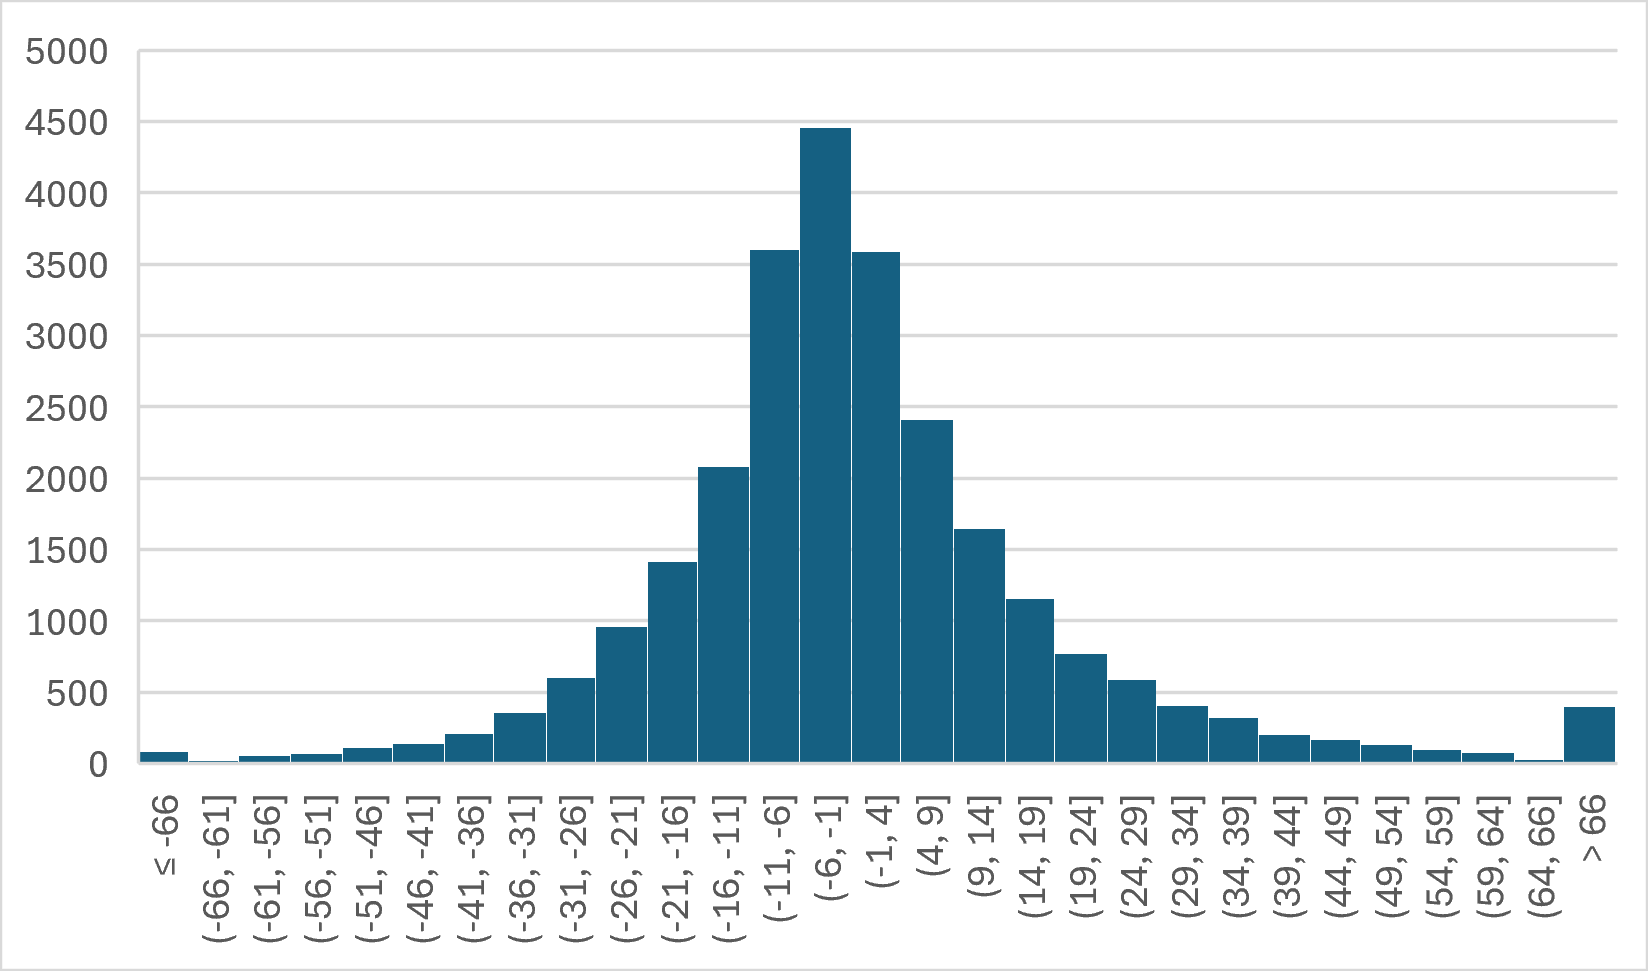
\includegraphics[width=1\linewidth]{Figures/histogram_average_realized_error.png}
    \caption{Histogram of the prediction error when using the historical average realized duration per surgery type.}
    \label{fig:hist_average_realized_error}
\end{figure}

\begin{figure}[h]
    \centering
    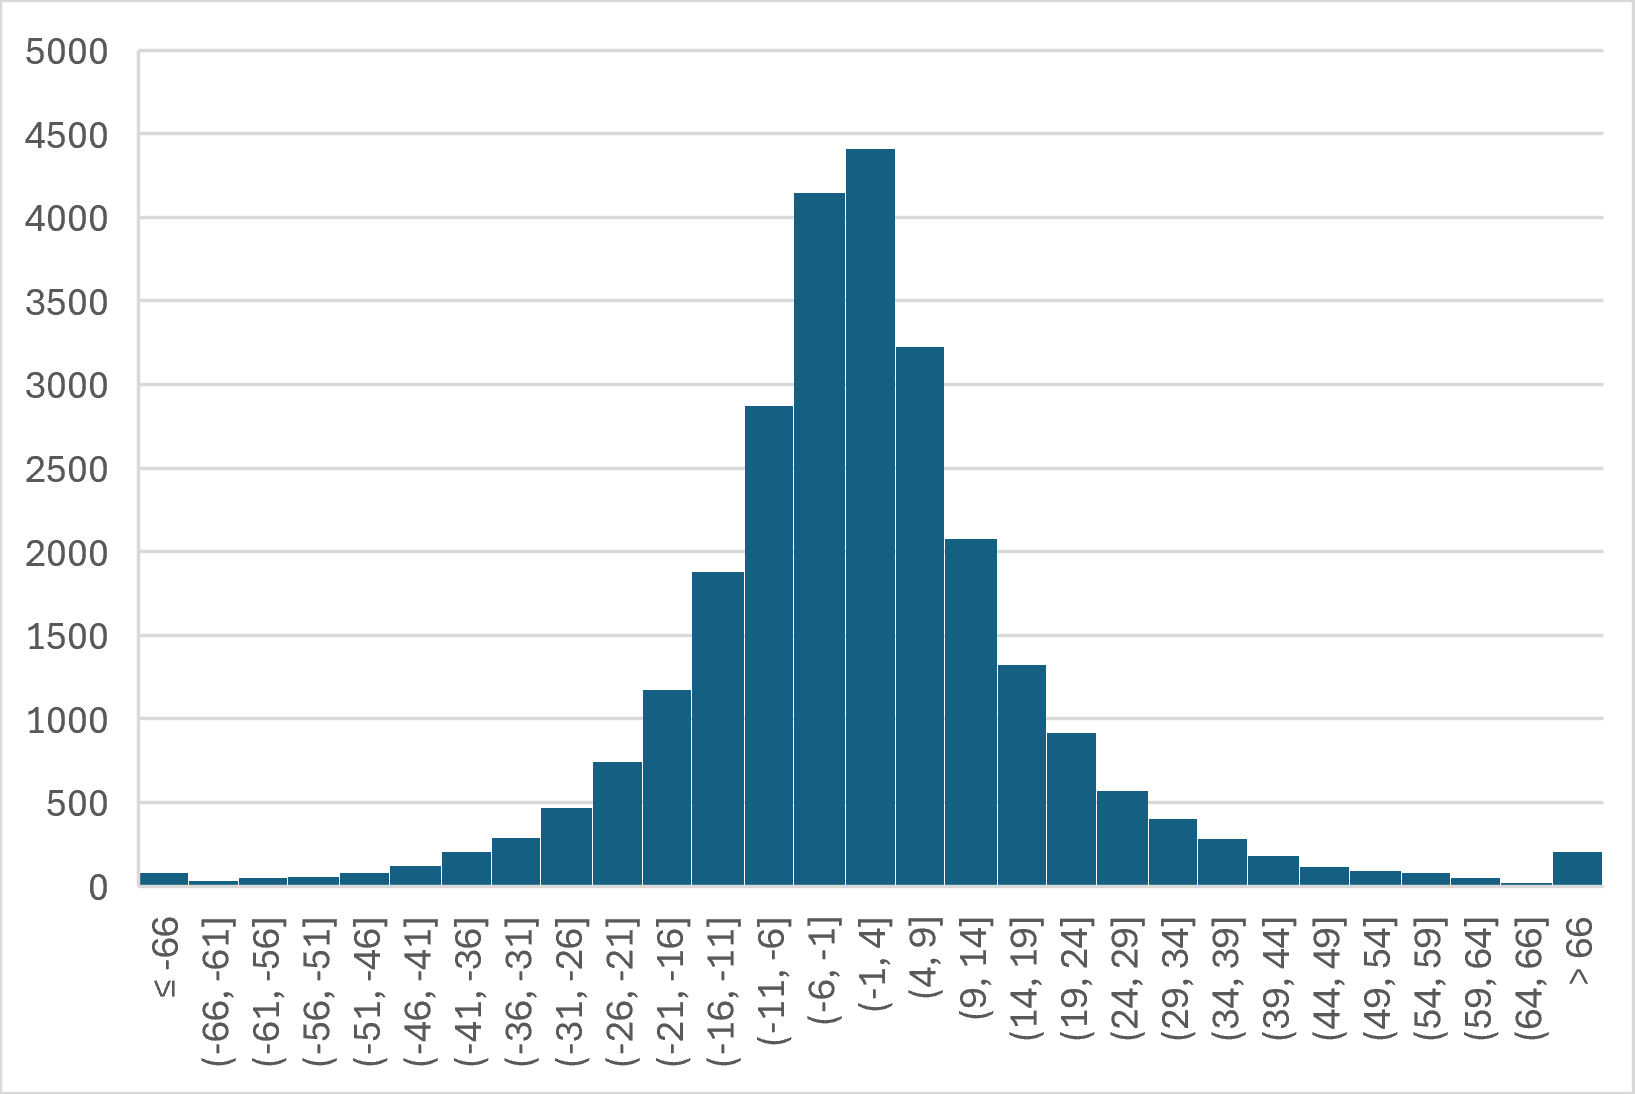
\includegraphics[width=1\linewidth]{Figures/histogram_planned_duration_error.png}
    \caption{Histogram of the prediction error when using the planned duration.}
    \label{fig:hist_planned_duration_error}
\end{figure}

\bibliographystyle{IEEEtran}
\bibliography{references}

\end{document}
